\documentclass[12pt,a4paper,oneside]{article}

% Pakiety i konfiguracje
\RequirePackage[utf8]{inputenc}
\usepackage[QX]{polski}
\usepackage[utf8]{inputenc}
\usepackage{latexsym}
\usepackage{tgpagella}
\usepackage{lmodern}
\usepackage{amsmath,amsthm,amsfonts,amssymb,alltt}
\usepackage{epsfig}
\usepackage{pdflscape}
\usepackage{caption}
\usepackage{indentfirst}
\usepackage{float}
\usepackage{listings}
\usepackage[polish]{babel}
\usepackage{datetime2}
\usepackage[x11names,dvipsnames,table]{xcolor}
\usepackage{hyperref}
\usepackage{underscore}
\usepackage{tikz}
\usepackage[linesnumbered,lined,commentsnumbered]{algorithm2e}
\usepackage{geometry}
\tolerance=1000
\hyphenpenalty=500

% Konfiguracja pakietu geometry
\geometry{
    a4paper,
    top=2.5cm,
    bottom=2.5cm,
    left=1.5cm,
    right=1.5cm,
    headheight=15pt, % dla nagłówków, jeśli są
    includehead,
    includefoot
}


\lstset{
  basicstyle=\ttfamily\small, % Czcionka dla kodu
  keywordstyle=\color{blue}\bfseries, % Styl dla słów kluczowych
  commentstyle=\color{gray}, % Styl dla komentarzy
  stringstyle=\color{red}, % Styl dla ciągów znaków
  breaklines=true, % Łamanie linii
  breakatwhitespace=true, % Łamanie linii w miejscu spacji
  frame=single, % Ramka wokół kodu
  captionpos=b, % Pozycja podpisu (b = poniżej)
  numbers=left, % Numery linii po lewej stronie
  numberstyle=\tiny\color{gray}, % Styl numerów linii
  showstringspaces=false, % Ukrywanie spacji w ciągach znaków
  escapeinside={(*@}{@*)}, % Używanie LaTeX w kodzie
}

% Konfiguracja listowania kodu HTML
\lstset{
  language=HTML, % Ustawienie języka na HTML
  basicstyle=\ttfamily\small, % Czcionka
  keywordstyle=\color{blue}\bfseries, % Kolor słów kluczowych
  commentstyle=\color{gray}, % Kolor komentarzy
  stringstyle=\color{red}, % Kolor ciągów znaków
  breaklines=true, % Łamanie linii
  breakatwhitespace=true, % Łamanie linii w miejscu spacji
  frame=single, % Ramka wokół kodu
  captionpos=b, % Podpis pod kodem
  numbers=left, % Numery linii po lewej
  numberstyle=\tiny\color{gray}, % Styl numerów linii
  showstringspaces=false, % Ukrywanie spacji w ciągach znaków
  escapeinside={(*@}{@*)} % Używanie LaTeX w listingu
}

% Specyficzne ustawienia dla języka Python
\lstdefinelanguage{Python}{
  keywords={def, return, if, elif, else, try, except, import, from, as, pass, break, continue, lambda, with, assert},
  keywordstyle=\color{blue}\bfseries,
  ndkeywords={self, True, False, None},
  ndkeywordstyle=\color{teal}\bfseries,
  identifierstyle=\color{black},
  sensitive=true,
  comment=[l]\#,
  morecomment=[s]{"""}{"""},
  commentstyle=\color{gray}\itshape,
  stringstyle=\color{red},
  morestring=[b]',
  morestring=[b]"
}

% Specyficzne ustawienia dla języka JavaScript
\lstdefinelanguage{JavaScript}{
  keywords={var, let, const, if, else, for, while, do, break, continue, return, switch, case, default, function, this, new, try, catch, finally, throw, class, extends, import, export, default, super, debugger},
  keywordstyle=\color{blue}\bfseries,
  ndkeywords={null, true, false, console, window, document},
  ndkeywordstyle=\color{teal}\bfseries,�cie�ka do sza-blonu u�y-wa-
  identifierstyle=\color{black},
  sensitive=true,
  comment=[l]//,
  morecomment=[s]{/*}{*/},
  commentstyle=\color{gray}\itshape,
  stringstyle=\color{red},
  morestring=[b]',
  morestring=[b]"
}


% Konfiguracja hyperref
\hypersetup{
    pdfauthor={Roman Czapla, Olaf Bar},
    colorlinks=True,
    linkcolor=darkgray,
    citecolor=BrickRed,
    filecolor=Magenta,
    urlcolor=BlueViolet
}

% Diagramy i algorytmy
\usetikzlibrary{positioning,arrows,chains,fit,shapes,calc}
\tikzset{main node/.style={circle,fill=blue!20,draw,minimum size=1cm,inner sep=0pt}}
\SetKwFor{ForEach}{for each}{do}{end for}%
\SetKwFor{ForAll}{for all}{do}{end for}%
\newenvironment{myalgorithm}
{\rule{\textwidth}{0.5mm}\\\SetAlCapSty{}\SetAlgoNoEnd\SetAlgoNoLine\begin{algorithm}}{\end{algorithm}\rule{\textwidth}{0.5mm}}

% Konfiguracja caption
\captionsetup{
    width=.95\linewidth,
    justification=centering
}

% Definicje matematyczne
\newtheorem{tw}{Twierdzenie}[section]
\newtheorem{lem}[tw]{Lemat}
\newtheorem{co}[tw]{Wniosek}
\newtheorem{prop}[tw]{Stwierdzenie}
\theoremstyle{definition}
\newtheorem{ex}{Przykład}
\newtheorem{re}[tw]{Uwaga}
\newtheorem{de}{Definicja}[section]

% Nowe komendy
\newcommand{\bC}{{\mathbb C}}
\newcommand{\bR}{{\mathbb R}}
\newcommand{\bZ}{{\mathbb Z}}
\newcommand{\bQ}{{\mathbb Q}}
\newcommand{\bN}{{\mathbb N}}
\newcommand{\captionT}[1]{\caption{\textsc{\footnotesize{#1}}}}
\renewcommand\figurename{Rys.}
\numberwithin{equation}{section}
\renewcommand{\thefootnote}{\arabic{footnote})}

\begin{document}
\renewcommand{\thepage}{\arabic{page}}
% --------------------------------------------
% Strona tytułowa
% --------------------------------------------

\thispagestyle{empty} % Ustawienie pustego stylu dla strony tytułowej
\begin{titlepage}
\begin{center}\Large
Uniwersytet Komisji Edukacji Narodowej w Krakowie\\
\large
Instytut Bezpieczeństwa i Informatyki\\
\vskip 10pt
\end{center}
\begin{center}
\centering 
\includegraphics[width=1.0\columnwidth]{images/logo.png}
\end{center}

\begin{center}
 {\bf \fontsize{14pt}{14pt}\selectfont PROJEKT INŻYNIERSKI \\ DOKUMENTACJA PROJEKTOWA}
\end{center}
\vskip 5pt
\begin{center}
 {\bf \fontsize{15pt}{25pt}\selectfont System rekomendacji produktów. Tworzenie algorytmu rekomendacyjnego na
 podstawie preferencji użytkowników – aplikacja przeglądarkowa}
\end{center}

\begin{center}
 {\fontsize{12pt}{12pt}\selectfont wykonany przez: }
\end{center}
\begin{center}
 {\bf\fontsize{16pt}{16pt}\selectfont Grzegorz x}\\
 {\fontsize{12pt}{12pt}\selectfont Nr albumu:  xxxx \\\&\\}
 {\bf\fontsize{16pt}{16pt}\selectfont Krzysztof x }\\
 {\fontsize{12pt}{12pt}\selectfont Nr albumu: x \\\&\\}
 {\bf\fontsize{16pt}{16pt}\selectfont Maciej x }\\
 {\fontsize{12pt}{12pt}\selectfont Nr albumu: x}
\end{center}
\begin{center}
 {\fontsize{12pt}{12pt}\selectfont pod opieką:}\\
 {\bf\fontsize{12pt}{12pt}\selectfont dr hab. inż.x x  }
\end{center}

\vspace*{\fill} % Dostosowanie dopełnienia do końca strony
\begin{center}
\large
Kraków \the\year\\
(ostatnia aktualizacja: \DTMcurrenttime,\;\today)
\end{center}
\end{titlepage}

\clearpage %

\tableofcontents


\newpage

\section{Szczegółowa dokumentacja projektowa}
\textit{W zależności od specyfiki projektu! Wymienione niżej podpunkty mają charakter orientacyjny.}
\subsection{Projekt UML}
\textit{W szczególności: diagram klas, ew. np. przypadki użycia, diagramy sekwencji, czynności, stanów, obiektów/komponentów/pakietów itp.}
\begin{center}
\centering 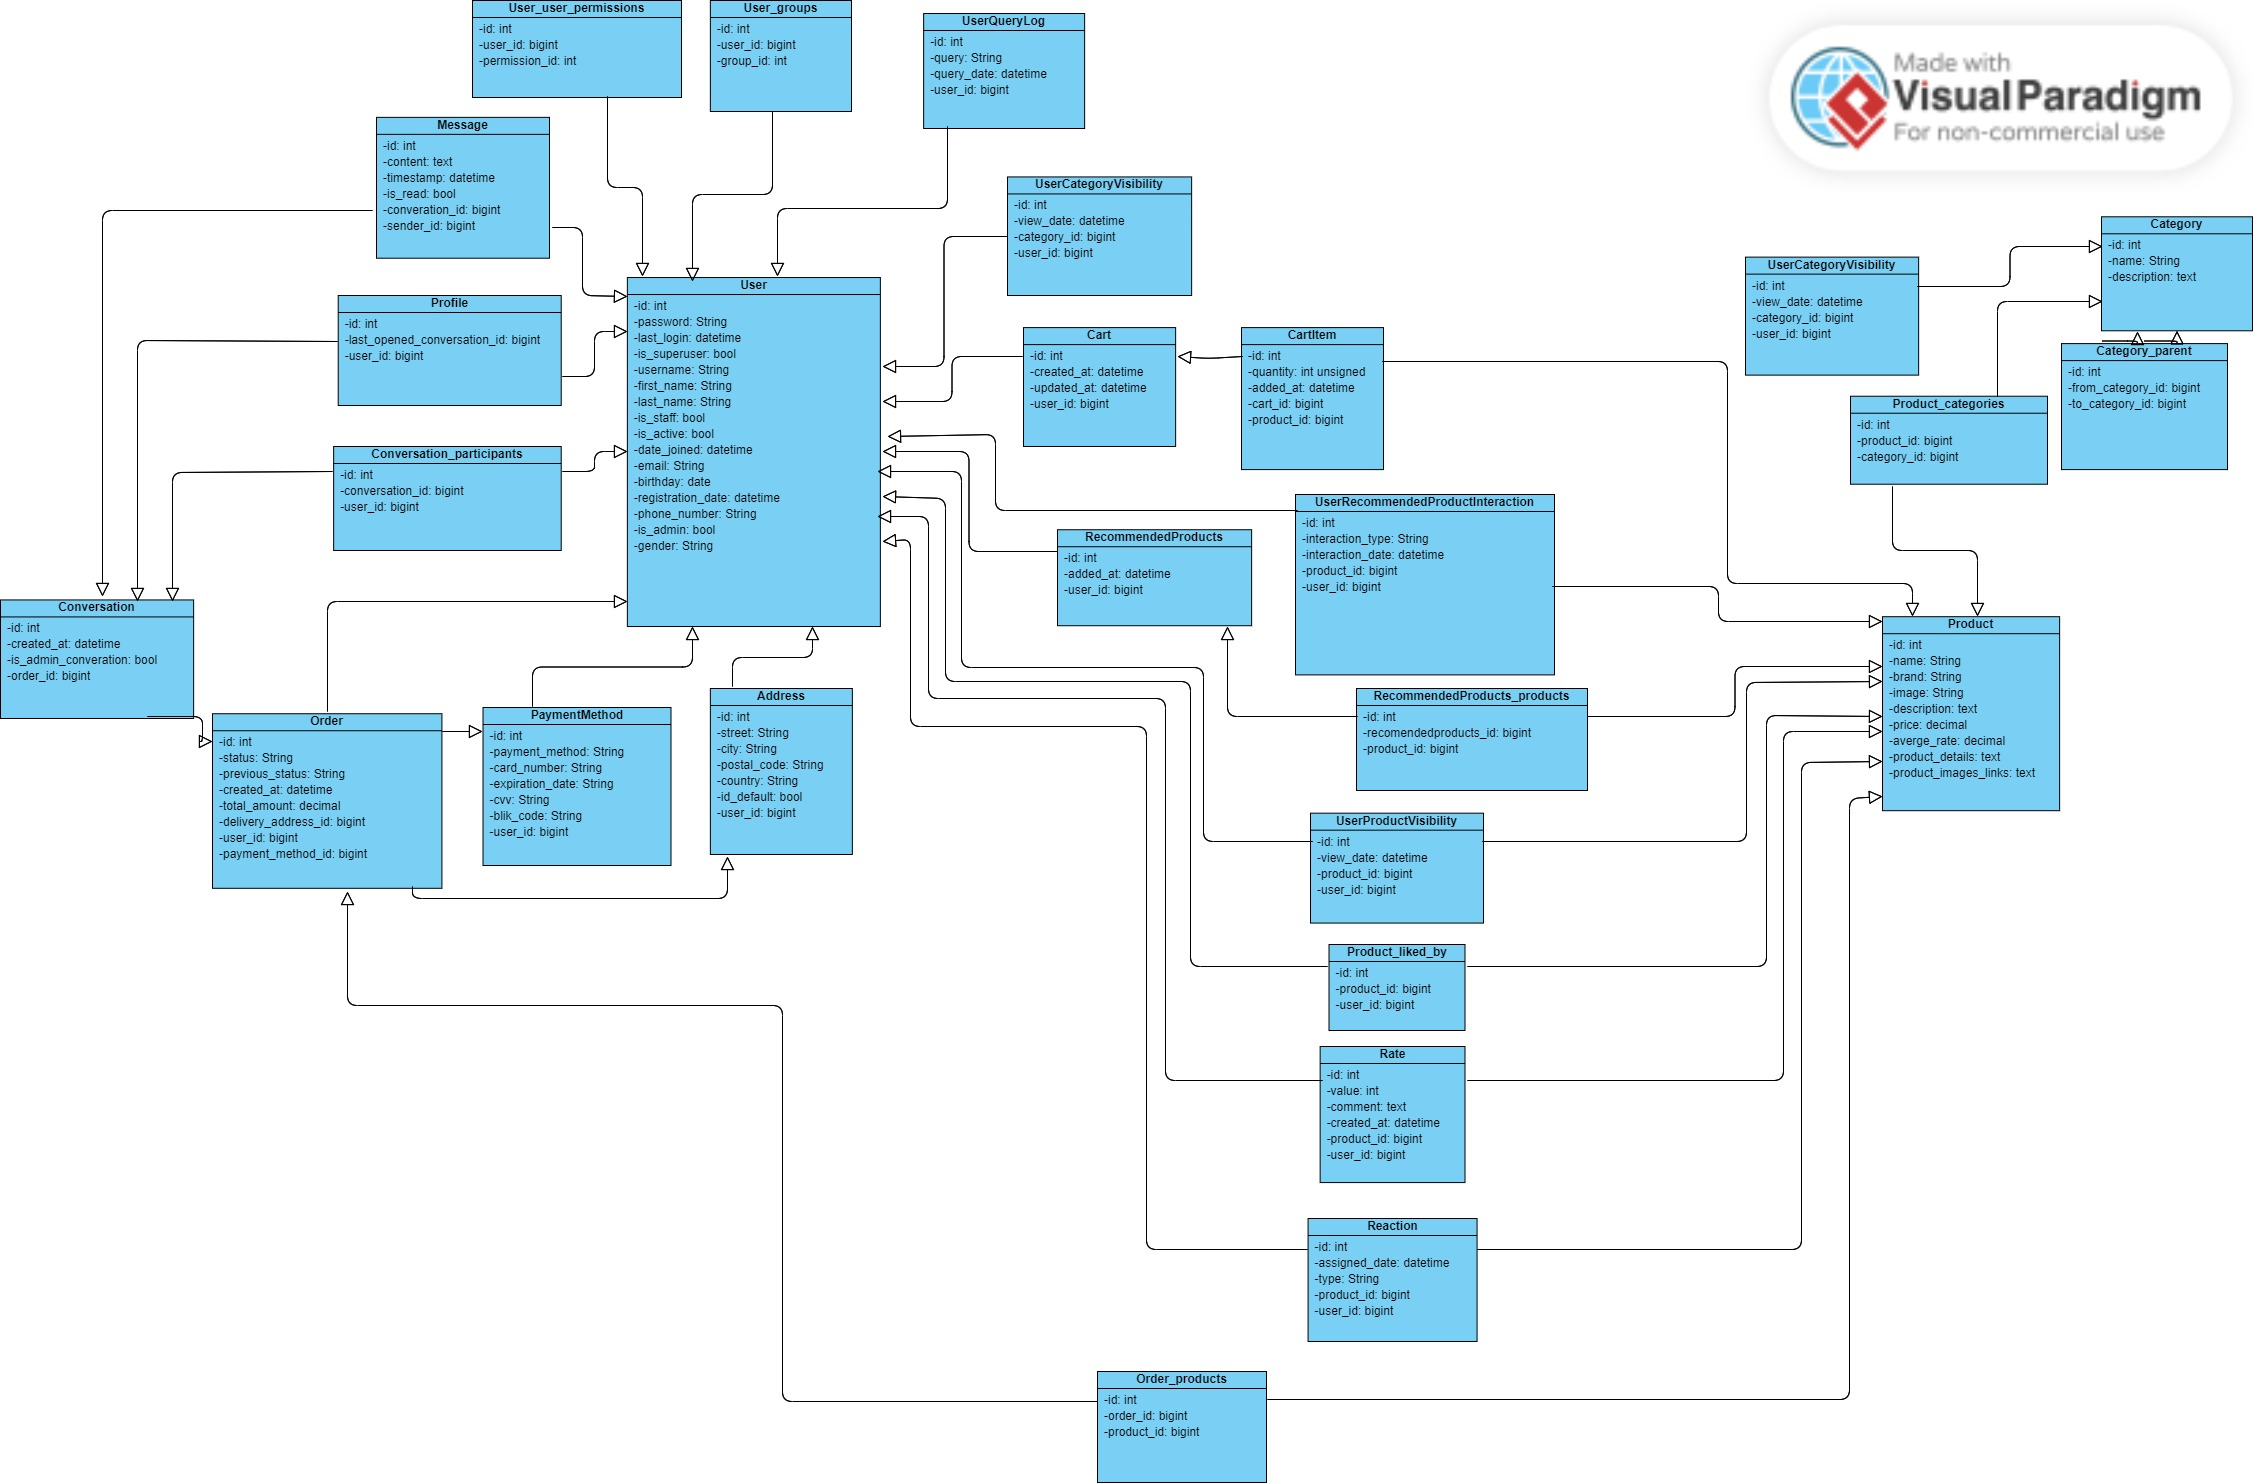
\includegraphics[width=1.0\columnwidth]{images/UML.jpg}
\end{center}

\subsection{Projekt bazy danych}

\subsubsection*{Tabela \texttt{Address}}
\textbf{Opis:} Przechowuje informacje o adresach użytkowników.
\begin{itemize}
    \item \texttt{street} : varchar(255) – ulica
    \item \texttt{city} : varchar(100) – miasto
    \item \texttt{postal\string_code} : varchar(20) – kod pocztowy
    \item \texttt{country} : varchar(100) – kraj
    \item \texttt{is\string_default} : bool – flaga domyślnego adresu
    \item \texttt{user\string_id} : bigint (klucz obcy do \texttt{User})
    \item \texttt{id} : integer (klucz główny)
\end{itemize}

\subsubsection*{Tabela \texttt{Cart}}
\textbf{Opis:} Przechowuje informacje o koszykach zakupowych.
\begin{itemize}
    \item \texttt{created\string_at} : datetime – data utworzenia koszyka
    \item \texttt{updated\string_at} : datetime – data ostatniej aktualizacji
    \item \texttt{user\string_id} : bigint (klucz obcy do \texttt{User})
    \item \texttt{id} : integer (klucz główny)
\end{itemize}

\subsubsection*{Tabela \texttt{CartItem}}
\textbf{Opis:} Przechowuje informacje o produktach w koszyku.
\begin{itemize}
    \item \texttt{quantity} : integer unsigned – ilość produktu
    \item \texttt{added\string_at} : datetime – data dodania produktu
    \item \texttt{cart\string_id} : bigint (klucz obcy do \texttt{Cart})
    \item \texttt{product\string_id} : bigint (klucz obcy do \texttt{Product})
    \item \texttt{id} : integer (klucz główny)
\end{itemize}

\subsubsection*{Tabela \texttt{Category}}
\textbf{Opis:} Przechowuje informacje o kategoriach produktów.
\begin{itemize}
    \item \texttt{name} : varchar(100) – nazwa kategorii
    \item \texttt{description} : text – opis kategorii
    \item \texttt{id} : integer (klucz główny)
\end{itemize}

\subsubsection*{Tabela \texttt{Category\string_parent}}
\textbf{Opis:} Definiuje relacje hierarchiczne między kategoriami.
\begin{itemize}
    \item \texttt{from\string_category\string_id} : bigint (klucz obcy do \texttt{Category})
    \item \texttt{to\string_category\string_id} : bigint (klucz obcy do \texttt{Category})
    \item \texttt{id} : integer (klucz główny)
\end{itemize}

\subsubsection*{Tabela \texttt{Conversation}}
\textbf{Opis:} Przechowuje informacje o rozmowach.
\begin{itemize}
    \item \texttt{created\string_at} : datetime – data utworzenia rozmowy
    \item \texttt{is\string_admin\string_conversation} : bool – flaga rozmowy administracyjnej
    \item \texttt{order\string_id} : bigint (klucz obcy do \texttt{Order})
    \item \texttt{id} : integer (klucz główny)
\end{itemize}

\subsubsection*{Tabela \texttt{Conversation\string_participants}}
\textbf{Opis:} Przechowuje uczestników rozmowy.
\begin{itemize}
    \item \texttt{conversation\string_id} : bigint (klucz obcy do \texttt{Conversation})
    \item \texttt{user\string_id} : bigint (klucz obcy do \texttt{User})
    \item \texttt{id} : integer (klucz główny)
\end{itemize}

\subsubsection*{Tabela \texttt{Message}}
\textbf{Opis:} Przechowuje wiadomości w rozmowach.
\begin{itemize}
    \item \texttt{content} : text – treść wiadomości
    \item \texttt{timestamp} : datetime – znacznik czasu wiadomości
    \item \texttt{is\string_read} : bool – flaga odczytania wiadomości
    \item \texttt{conversation\string_id} : bigint (klucz obcy do \texttt{Conversation})
    \item \texttt{sender\string_id} : bigint (klucz obcy do \texttt{User})
    \item \texttt{id} : integer (klucz główny)
\end{itemize}

\subsubsection*{Tabela \texttt{Order}}
\textbf{Opis:} Przechowuje informacje o zamówieniach.
\begin{itemize}
    \item \texttt{status} : varchar(20) – status zamówienia
    \item \texttt{previous\string_status} : varchar(20) – poprzedni status
    \item \texttt{created\string_at} : datetime – data utworzenia
    \item \texttt{total\string_amount} : decimal – łączna kwota
    \item \texttt{delivery\string_address\string_id} : bigint (klucz obcy do \texttt{Address})
    \item \texttt{user\string_id} : bigint (klucz obcy do \texttt{User})
    \item \texttt{payment\string_method\string_id} : bigint (klucz obcy do \texttt{PaymentMethod})
    \item \texttt{id} : integer (klucz główny)
\end{itemize}

\subsubsection*{Tabela \texttt{PaymentMethod}}
\textbf{Opis:} Przechowuje informacje o metodach płatności.
\begin{itemize}
    \item \texttt{payment\string_method} : varchar(20) – typ metody
    \item \texttt{card\string_number} : varchar(16) – numer karty
    \item \texttt{expiration\string_date} : varchar(5) – data ważności
    \item \texttt{cvv} : varchar(4) – kod CVV
    \item \texttt{blik\string_code} : varchar(6) – kod Blik
    \item \texttt{user\string_id} : bigint (klucz obcy do \texttt{User})
    \item \texttt{id} : integer (klucz główny)
\end{itemize}

\subsubsection*{Tabela \texttt{Product}}
\textbf{Opis:} Przechowuje informacje o produktach.
\begin{itemize}
    \item \texttt{name} : varchar(100) – nazwa produktu
    \item \texttt{brand} : varchar(100) – marka produktu
    \item \texttt{image} : varchar(100) – obraz produktu
    \item \texttt{description} : text – opis produktu
    \item \texttt{price} : decimal – cena produktu
    \item \texttt{average\string_rate} : decimal – średnia ocena
    \item \texttt{product\string_details} : text – szczegóły produktu
    \item \texttt{product\string_images\string_links} : text – linki do zdjęć
    \item \texttt{id} : integer (klucz główny)
\end{itemize}

\subsubsection*{Tabela \texttt{Order\string_products}}
\textbf{Opis:} Przechowuje informacje o produktach w zamówieniach.
\begin{itemize}
    \item \texttt{order\string_id} : bigint (klucz obcy do \texttt{Order})
    \item \texttt{product\string_id} : bigint (klucz obcy do \texttt{Product})
    \item \texttt{id} : integer (klucz główny)
\end{itemize}

\subsubsection*{Tabela \texttt{Product\string_categories}}
\textbf{Opis:} Przechowuje relacje między produktami a kategoriami.
\begin{itemize}
    \item \texttt{product\string_id} : bigint (klucz obcy do \texttt{Product})
    \item \texttt{category\string_id} : bigint (klucz obcy do \texttt{Category})
    \item \texttt{id} : integer (klucz główny)
\end{itemize}

\subsubsection*{Tabela \texttt{Product\string_liked\string_by}}
\textbf{Opis:} Przechowuje informacje o użytkownikach, którzy polubili produkty.
\begin{itemize}
    \item \texttt{product\string_id} : bigint (klucz obcy do \texttt{Product})
    \item \texttt{user\string_id} : bigint (klucz obcy do \texttt{User})
    \item \texttt{id} : integer (klucz główny)
\end{itemize}

\subsubsection*{Tabela \texttt{RecommendedProducts}}
\textbf{Opis:} Przechowuje listy rekomendowanych produktów.
\begin{itemize}
    \item \texttt{added\string_at} : datetime – data dodania listy
    \item \texttt{user\string_id} : bigint (klucz obcy do \texttt{User})
    \item \texttt{id} : integer (klucz główny)
\end{itemize}

\subsubsection*{Tabela \texttt{RecommendedProducts\string_products}}
\textbf{Opis:} Przechowuje produkty powi\k{a}zane z rekomendacjami.
\begin{itemize}
    \item \texttt{RecommendedProducts\string_id} : bigint (klucz obcy do \texttt{RecommendedProducts})
    \item \texttt{product\string_id} : bigint (klucz obcy do \texttt{Product})
    \item \texttt{id} : integer (klucz główny)
\end{itemize}

\subsubsection*{Tabela \texttt{User\string_groups}}
\textbf{Opis:} Przechowuje relacje między użytkownikami a grupami.
\begin{itemize}
    \item \texttt{user\string_id} : bigint (klucz obcy do \texttt{User})
    \item \texttt{group\string_id} : integer (klucz obcy do \texttt{Auth\string_group})
    \item \texttt{id} : integer (klucz główny)
\end{itemize}

\subsubsection*{Tabela \texttt{UserCategoryVisibility}}
\textbf{Opis:} Przechowuje informacje o widoczności kategorii dla użytkowników.
\begin{itemize}
    \item \texttt{view\string_date} : datetime – data widoczności
    \item \texttt{category\string_id} : bigint (klucz obcy do \texttt{Category})
    \item \texttt{user\string_id} : bigint (klucz obcy do \texttt{User})
    \item \texttt{id} : integer (klucz główny)
\end{itemize}

\subsubsection*{Tabela \texttt{UserQueryLog}}
\textbf{Opis:} Przechowuje zapytania wykonane przez użytkowników.
\begin{itemize}
    \item \texttt{query} : varchar(255) – treść zapytania
    \item \texttt{query\string_date} : datetime – data zapytania
    \item \texttt{user\string_id} : bigint (klucz obcy do \texttt{User})
    \item \texttt{id} : integer (klucz główny)
\end{itemize}

\subsubsection*{Tabela \texttt{Profile}}
\textbf{Opis:} Przechowuje informacje o profilach użytkowników.
\begin{itemize}
    \item \texttt{last\string_opened\string_conversation\string_id} : bigint (klucz obcy do \texttt{Conversation})
    \item \texttt{user\string_id} : bigint (klucz obcy do \texttt{User})
    \item \texttt{id} : integer (klucz główny)
\end{itemize}

\subsubsection*{Tabela \texttt{Rate}}
\textbf{Opis:} Przechowuje oceny produktów wystawione przez użytkowników.
\begin{itemize}
    \item \texttt{value} : integer – wartość oceny
    \item \texttt{comment} : text – komentarz do oceny
    \item \texttt{created\string_at} : datetime – data wystawienia oceny
    \item \texttt{product\string_id} : bigint (klucz obcy do \texttt{Product})
    \item \texttt{user\string_id} : bigint (klucz obcy do \texttt{User})
    \item \texttt{id} : integer (klucz główny)
\end{itemize}

\subsubsection*{Tabela \texttt{Reaction}}
\textbf{Opis:} Przechowuje reakcje użytkowników na produkty.
\begin{itemize}
    \item \texttt{assigned\string_date} : datetime – data przypisania reakcji
    \item \texttt{type} : varchar(10) – typ reakcji (np. „like” lub „dislike”)
    \item \texttt{product\string_id} : bigint (klucz obcy do \texttt{Product})
    \item \texttt{user\string_id} : bigint (klucz obcy do \texttt{User})
    \item \texttt{id} : integer (klucz główny)
\end{itemize}

\subsubsection*{Tabela \texttt{UserProductVisibility}}
\textbf{Opis:} Przechowuje informacje o widoczności produktów dla użytkowników.
\begin{itemize}
    \item \texttt{view\string_date} : datetime – data widoczności
    \item \texttt{product\string_id} : bigint (klucz obcy do \texttt{Product})
    \item \texttt{user\string_id} : bigint (klucz obcy do \texttt{User})
    \item \texttt{id} : integer (klucz główny)
\end{itemize}

\subsubsection*{Tabela \texttt{UserRecommendedProductInteraction}}
\textbf{Opis:} Przechowuje informacje o interakcjach użytkowników z rekomendowanymi produktami.
\begin{itemize}
    \item \texttt{interaction\string_type} : varchar(20) – typ interakcji (np. kliknięcie, zakup)
    \item \texttt{interaction\string_date} : datetime – data interakcji
    \item \texttt{product\string_id} : bigint (klucz obcy do \texttt{Product})
    \item \texttt{user\string_id} : bigint (klucz obcy do \texttt{User})
    \item \texttt{id} : integer (klucz główny)
\end{itemize}

\subsubsection*{Tabela \texttt{User\string_user\string_permissions}}
\textbf{Opis:} Przechowuje informacje o uprawnieniach użytkowników.
\begin{itemize}
    \item \texttt{user\string_id} : bigint (klucz obcy do \texttt{User})
    \item \texttt{permission\string_id} : integer (klucz obcy do \texttt{Auth\string_permission})
    \item \texttt{id} : integer (klucz główny)
\end{itemize}

\subsubsection*{Tabela \texttt{User\string_query\string_log}}
\textbf{Opis:} Przechowuje zapytania wyszukiwania wykonane przez użytkowników.
\begin{itemize}
    \item \texttt{query} : varchar(255) – treść zapytania
    \item \texttt{query\string_date} : datetime – data zapytania
    \item \texttt{user\string_id} : bigint (klucz obcy do \texttt{User})
    \item \texttt{id} : integer (klucz główny)
\end{itemize}


\section*{Relacje między tabelami}
\begin{itemize}
    \item \texttt{Address.user\string_id} $\to$ \texttt{User.id}
    \item \texttt{Cart.user\string_id} $\to$ \texttt{User.id}
    \item \texttt{CartItem.cart\string_id} $\to$ \texttt{Cart.id}
    \item \texttt{CartItem.product\string_id} $\to$ \texttt{Product.id}
    \item \texttt{Category\string_parent.from\string_category\string_id} $\to$ \texttt{Category.id}
    \item \texttt{Category\string_parent.to\string_category\string_id} $\to$ \texttt{Category.id}
    \item \texttt{Conversation.order\string_id} $\to$ \texttt{Order.id}
    \item \texttt{Conversation\string_participants.conversation\string_id} $\to$ \texttt{Conversation.id}
    \item \texttt{Conversation\string_participants.user\string_id} $\to$ \texttt{User.id}
    \item \texttt{Message.conversation\string_id} $\to$ \texttt{Conversation.id}
    \item \texttt{Message.sender\string_id} $\to$ \texttt{User.id}
    \item \texttt{Order\string_products.order\string_id} $\to$ \texttt{Order.id}
    \item \texttt{Order\string_products.product\string_id} $\to$ \texttt{Product.id}
    \item \texttt{Product\string_categories.product\string_id} $\to$ \texttt{Product.id}
    \item \texttt{Product\string_categories.category\string_id} $\to$ \texttt{Category.id}
    \item \texttt{Product\string_liked\string_by.product\string_id} $\to$ \texttt{Product.id}
    \item \texttt{Product\string_liked\string_by.user\string_id} $\to$ \texttt{User.id}
    \item \texttt{RecommendedProducts\string_products.recommendedproducts\string_id} $\to$ \texttt{RecommendedProducts.id}
    \item \texttt{RecommendedProducts\string_products.product\string_id} $\to$ \texttt{Product.id}
    \item \texttt{User\string_groups.user\string_id} $\to$ \texttt{User.id}
    \item \texttt{UserCategoryVisibility.category\string_id} $\to$ \texttt{Category.id}
    \item \texttt{Profile.last\string_opened\string_conversation\string_id} $\to$ \texttt{Conversation.id}
    \item \texttt{Rate.product\string_id} $\to$ \texttt{Product.id}
    \item \texttt{Rate.user\string_id} $\to$ \texttt{User.id}
    \item \texttt{Reaction.product\string_id} $\to$ \texttt{Product.id}
    \item \texttt{Reaction.user\string_id} $\to$ \texttt{User.id}
    \item \texttt{UserRecommendedProductInteraction.product\string_id} $\to$ \texttt{Product.id}
    \item \texttt{UserRecommendedProductInteraction.user\string_id} $\to$ \texttt{User.id}
\end{itemize}


\subsubsection*{Przykładowe procedury składowane}

\subsubsection*{Dodawanie nowego użytkownika}
\begin{verbatim}
CREATE OR REPLACE PROCEDURE add_user(
    p_username VARCHAR,
    p_email VARCHAR,
    p_password VARCHAR
)
BEGIN
    INSERT INTO User (username, email, password)
    VALUES (p_username, p_email, p_password);
END;
\end{verbatim}

\subsubsection*{Pobieranie zamówień użytkownika}
\begin{verbatim}
CREATE OR REPLACE FUNCTION get_user_orders(p_user_id INT)
RETURNS TABLE(order_id INT, order_date DATETIME, status VARCHAR)
BEGIN
    RETURN QUERY
    SELECT id, order_date, status
    FROM Order
    WHERE user_id = p_user_id;
END;
\end{verbatim}

\clearpage
\subsection{Szczegółowa dokumentacja kodu}
Poniżej przedstawiono szczegółową dokumentację dotyczącą implementacji aplikacji. Dokumentacja obejmuje:
\begin{itemize}
\item \textit{opis najważniejszych zmiennych;}
\item \textit{specyfikacja i opis wszystkich klas (jeśli projekt obiektowy) - opis całej klasy, jej pól i metod (jak poniżej);}
\item \textit{opis funkcji oraz metod klas (co robią, opis poszczególnych parametrów wejściowych i zwracanych wartości itp.) oraz w przypadku bibliotek programistycznych - przykłady użycia (przykładowy kod);} 
\item \textit{opis użytych wzorców projektowych.}
\end{itemize}
% User Model details documentation 
\subsubsection{Model \texttt{User}}
\textbf{Opis:} 
Model \texttt{User} rozszerza wbudowany model \texttt{AbstractUser} i przechowuje informacje o użytkownikach systemu, takie jak dane personalne, datę rejestracji, numer telefonu oraz płeć. Wprowadza dodatkowe pola, które uzupełniają funkcjonalności dziedziczone z \texttt{AbstractUser}.

\textbf{Pola dodane w modelu \texttt{User}:}
\begin{itemize}
    \item \texttt{email}: \texttt{EmailField} – unikalny adres e-mail użytkownika (nadpisuje pole z \texttt{AbstractUser}).
    \item \texttt{birthday}: \texttt{DateField} – data urodzenia użytkownika (opcjonalne).
    \item \texttt{registration\_date}: \texttt{DateTimeField} – data rejestracji użytkownika (domyślnie ustawiana na bieżącą datę i czas).
    \item \texttt{phone\_number}: \texttt{CharField} – numer telefonu użytkownika (wymagane, maksymalnie 15 znaków).
    \item \texttt{is\_admin}: \texttt{BooleanField} – flaga wskazująca, czy użytkownik jest administratorem.
    \item \texttt{gender}: \texttt{CharField} – płeć użytkownika, wybierana spośród wartości:
    \begin{itemize}
        \item \texttt{Male}
        \item \texttt{Female}
        \item \texttt{Other}
    \end{itemize}
\end{itemize}

\textbf{Pola dziedziczone z modelu \texttt{AbstractUser}:}
\begin{itemize}
    \item \texttt{password}: \texttt{CharField} – hasło użytkownika (zabezpieczone poprzez funkcję \texttt{set\_password}).
    \item \texttt{last\_login}: \texttt{DateTimeField} – data ostatniego logowania użytkownika.
    \item \texttt{is\_superuser}: \texttt{BooleanField} – flaga oznaczająca, czy użytkownik jest superużytkownikiem.
    \item \texttt{username}: \texttt{CharField} – unikalna nazwa użytkownika.
    \item \texttt{first\_name}: \texttt{CharField} – imię użytkownika.
    \item \texttt{last\_name}: \texttt{CharField} – nazwisko użytkownika.
    \item \texttt{is\_staff}: \texttt{BooleanField} – flaga wskazująca, czy użytkownik ma uprawnienia do panelu administracyjnego.
    \item \texttt{is\_active}: \texttt{BooleanField} – flaga wskazująca, czy konto użytkownika jest aktywne.
    \item \texttt{date\_joined}: \texttt{DateTimeField} – data utworzenia konta użytkownika.
\end{itemize}

\subsubsection*{Metody modelu}
\begin{itemize}
    \item \texttt{\_\_str\_\_(self)}:
    \begin{itemize}
        \item \textbf{Opis:} Zwraca czytelną reprezentację użytkownika w formacie: \\
        \texttt{User <imie> <nazwisko> <email> \ Gender: <płeć>}.
        \item \textbf{Przykład:}
        \begin{lstlisting}
    user = User.objects.get(id=1)
    print(user)  # Output: User John Doe john.doe@example.com Gender: Male
        \end{lstlisting}
    \end{itemize}
\end{itemize}

\subsubsection*{Formularze związane z modelem}

\paragraph{Formularz rejestracji (\texttt{UserRegistrationForm})}

\begin{itemize}
    \item \textbf{Opis:} Formularz umożliwiający rejestrację nowego użytkownika w systemie.
    \item \textbf{Pola:} 
    \begin{itemize}
        \item \texttt{first\_name}, \texttt{last\_name}, \texttt{email}, \texttt{phone\_number}, \texttt{birthday}, \texttt{gender}, \texttt{password}.
    \end{itemize}
    % Metody walidacji 
    \subsubsection*{Metody walidacji formularza}
    \begin{itemize}
        %  Metoda clean_email
        \item \texttt{clean\_email}
        \begin{itemize}
            \item \textbf{Opis:} Sprawdza, czy adres e-mail jest unikalny i należy do poprawnej domeny.
            \item \textbf{Kod:}
            \begin{lstlisting}[language=Python, caption=Kod metody clean\_email]
def clean_email(self):
    email = self.cleaned_data.get("email")
    if User.objects.filter(email=email).exists():
        raise forms.ValidationError(f"Email is already taken")
    elif "@" in email:
        domain = email.split("@")[1]
        if domain.split(".")[-1] not in POSSIBLE_EMAIL_DOMAIN_TLD:
            raise forms.ValidationError("Given email domain not recognized")
    return email
        \end{lstlisting}
        \item \textbf{Przykład:}
        \begin{verbatim}
Input: email = "invalid_domain@fake_domain.notreal"
Output: ValidationError: "Given email domain not recognized"
            \end{verbatim}
        \end{itemize}
    
        %  Metoda clean_phone_number
        \item \texttt{clean\_phone\_number}
        \begin{itemize}
            \item \textbf{Opis:} Upewnia się, że numer telefonu zawiera dokładnie 9 cyfr.
            \item \textbf{Kod:}
            \begin{lstlisting}[language=Python, caption=Kod metody clean\_phone\_number]
def clean_phone_number(self):
    phone_number = self.cleaned_data.get("phone_number")
    parsed_phone_number = re.sub(r'\D', '', phone_number)
    if len(parsed_phone_number) != 9:
        raise ValidationError("Phone number must have exactly 9 digits.")
    return parsed_phone_number
        \end{lstlisting}
        \item \textbf{Przykład:}
        \begin{verbatim}
Input: phone_number = "+48 123-456-789"
Output: "123456789"
            \end{verbatim}
        \end{itemize}
    \end{itemize}
\clearpage % mowing to other page 
    \item \textbf{Metody:}
    \item \texttt{generate\_username(first\_name, last\_name)}
    \begin{itemize}
        \item \textbf{Opis:} Generuje unikalną nazwę użytkownika na podstawie imienia i nazwiska. Jeśli istnieje już użytkownik o takiej nazwie, metoda dodaje liczbę do nazwy, aby zapewnić jej unikalność.
        \item \textbf{Kod:}
        \begin{lstlisting}[language=Python, caption=Kod metody generate\_username]
@staticmethod
def generate_username(first_name, last_name):
    first_name = first_name.lower()
    last_name = last_name.lower()

    if " " in first_name:
        first_name = "_".join(first_name.split())
    if " " in last_name:
        last_name = "_".join(last_name.split())

    username = f"{first_name}.{last_name}"
    num = 1

    while User.objects.filter(username=username).exists():
        username = f"{first_name}.{last_name}{num}"
        num += 1

    return username
        \end{lstlisting}
        \item \textbf{Przykład:}
        \begin{verbatim}
    Input: first_name = "John", last_name = "Doe"
    Output: "john.doe"

    Input: first_namqe = "John", last_name = "Doe" (if "john.doe" already exists)
    Output: "john.doe1"
        \end{verbatim}
    \end{itemize}
\end{itemize}

% \clearpage % mowing to other page 
\paragraph{Formularz logowania (\texttt{UserLoginForm})}

\begin{itemize}
    \item \textbf{Opis:} Formularz umożliwiający logowanie użytkownika na podstawie adresu e-mail i hasła.
    \item \textbf{Pola:}
    \begin{itemize}
        \item \texttt{email}, \texttt{password}.
    \end{itemize}
\end{itemize}

\subsubsection*{Widoki związane z modelem}

\paragraph{\texttt{UserRegisterView}}
\begin{itemize}
    \item \textbf{Opis:} Widok umożliwiający użytkownikom rejestrację w systemie.
    \item \textbf{Atrybuty:}
    \begin{itemize}
        \item \texttt{template\_name}: Ścieżka do szablonu używanego dla rejestracji (\texttt{"registration/register.html"}). 
        Kod szablonu został szczegółowo opisany w sekcji \ref{sec:register_template}.
        \item \texttt{form\_class}: Formularz używany w widoku rejestracji (\texttt{UserRegistrationForm}).
        \item \texttt{success\_url}: URL, na który użytkownik jest przekierowywany po pomyślnej rejestracji (\texttt{"login"}).
    \end{itemize}
    \item \textbf{Metody:}
    \begin{itemize}
        \item \texttt{form\_valid(self, form)}:
        \begin{itemize}
            \item \textbf{Opis:} Obsługuje poprawne przesłanie formularza rejestracji.
            \item \textbf{Kod:}
            \begin{lstlisting}[language=Python, caption=Metoda form\_valid w UserRegisterView]
def form_valid(self, form):
    form.save(commit=True)
    messages.success(self.request, "Registered successfully")
    send_registration_email(form.cleaned_data['email'], form.cleaned_data['first_name'])
    return super().form_valid(form)
            \end{lstlisting}
            \item \textbf{Wyjaśnienie:}
            \begin{itemize}
                \item Zapisuje nowego użytkownika w bazie danych.
                \item Wyświetla komunikat o sukcesie przy użyciu systemu wiadomości Django.
                \item Wysyła e-mail z potwierdzeniem rejestracji na adres użytkownika.  (szczegóły funkcji \texttt{send\_registration\_email} w sekcji \ref{sec:helper_functions}).
            \end{itemize}
        \end{itemize}
        \item \texttt{form\_invalid(self, form)}:
        \begin{itemize}
            \item \textbf{Opis:} Obsługuje niepoprawne przesłanie formularza.
            \item \textbf{Kod:}
            \begin{lstlisting}[language=Python, caption=Metoda form\_invalid w UserRegisterView]
def form_invalid(self, form):
    return super().form_invalid(form)
            \end{lstlisting}
            \item \textbf{Wyjaśnienie:}
            \begin{itemize}
                \item Przekazuje niepoprawny formularz do szablonu w celu wyświetlenia błędów.
            \end{itemize}
        \end{itemize}
    \end{itemize}
\end{itemize}

\paragraph{\texttt{UserLoginView}}
\begin{itemize}
    \item \textbf{Opis:} Widok umożliwiający logowanie użytkownika.
    \item \textbf{Atrybuty:}
    \begin{description}
        \item[\texttt{template\_name}] Ścieżka do szablonu logowania (\texttt{"registration/login.html"}).\\
        \hspace{1cm} Kod szablonu został szczegółowo opisany w sekcji \ref{sec:login_template}.
        \item[\texttt{form\_class}] Formularz używany w widoku logowania (\texttt{UserLoginForm}).
        \item[\texttt{success\_url}] URL, na który użytkownik jest przekierowywany po pomyślnym zalogowaniu (\texttt{"home"}).
    \end{description}
    \item \textbf{Metody:}
    \begin{itemize}
    \item \texttt{form\_valid(self, form)}:
    \begin{itemize}
        \item \textbf{Opis:} Obsługuje poprawne przesłanie formularza logowania.
        \item \textbf{Kod:}
        \begin{lstlisting}[language=Python, caption=Metoda form\_valid w UserLoginView]
def form_valid(self, form):
    email = form.cleaned_data.get('email')
    password = form.cleaned_data.get('password')
    try:
        user = User.objects.get(email=email)
        username = user.username
        user = authenticate(self.request, username=username, password=password)
        if user is not None:
            login(self.request, user)
            messages.success(self.request, "Login successfully")
            sync_session_likes_to_user(self.request)
            return super().form_valid(form)
        else:
            form.add_error(None, "Incorrect email or password")
    except User.DoesNotExist:
        form.add_error('email', "No user found with the given email address")
    return self.form_invalid(form)
            \end{lstlisting}
            \item \textbf{Wyjaśnienie:}
            \begin{itemize}
                \item Pobiera dane logowania z formularza (\texttt{email}, \texttt{password}).
                \item Wyszukuje użytkownika na podstawie adresu e-mail.
                \item Próbuje uwierzytelnić użytkownika za pomocą funkcji \texttt{authenticate}.
                \item Jeśli uwierzytelnienie powiedzie się, loguje użytkownika i wyświetla komunikat o sukcesie.
                \item Jeśli uwierzytelnienie nie powiedzie się, dodaje odpowiednie błędy do formularza.
            \end{itemize}
        \end{itemize}
    \end{itemize}
\end{itemize}


\subsubsection*{Endpointy związane z modelem}

\begin{itemize}
    \item \texttt{/register/} – rejestracja użytkownika (\texttt{UserRegisterView}).
    \item \texttt{/login/} – logowanie użytkownika (\texttt{UserLoginView}).
    \item \texttt{/logout/} – wylogowanie użytkownika (\texttt{logout\_view}).
\end{itemize}

\subsubsection*{Szablony użytkownika}
\label{sec:user_templates}

\paragraph{\texttt{login.html}}
\label{sec:login_template}

Szablon odpowiedzialny za logowanie użytkownika do systemu. Poniżej przedstawiono fragment kodu HTML użytego w szablonie:

\begin{lstlisting}[language=HTML, caption=Szablon login.html]
    <form method="post" action="">
        
        <label for="id_email">Email:</label>
        <input type="email" name="email" id="id_email" required>
        <label for="id_password">Haslo:</label>
        <input type="password" name="password" id="id_password" required>
        <button type="submit">Zaloguj sie</button>
    </form>
\end{lstlisting}

\textbf{Wyjaśnienie:}
\begin{itemize}
    \item \texttt{method="post"}: Określa metodę przesyłania danych (HTTP POST).
    \item \texttt{{\% csrf\_token \%}}: Token zabezpieczający przed atakami CSRF (wymagany w Django).
    \item \texttt{name="email"}: Pole do wprowadzenia adresu e-mail.
    \item \texttt{name="password"}: Pole do wprowadzenia hasła użytkownika.
    \item Przycisk \texttt{submit}: Służy do przesłania formularza do widoku logowania.
\end{itemize}

\begin{figure}[H] % 'H' wymusza umieszczenie w bieżącym miejscu
    \paragraph{\texttt{register.html}}
    \label{sec:register_template}
    Szablon odpowiedzialny za rejestrację nowych użytkowników. Poniżej przedstawiono fragment kodu HTML użytego w szablonie:
    \begin{lstlisting}[language=HTML, caption=Szablon register.html]
        <form method="post" action="">
            
            <label for="id_first_name">Imie:</label>
            <input type="text" name="first_name" id="id_first_name" required>
            <label for="id_last_name">Nazwisko:</label>
            <input type="text" name="last_name" id="id_last_name" required>
            <label for="id_email">Email:</label>
            <input type="email" name="email" id="id_email" required>
            <button type="submit">Zarejestruj sie</button>
        </form>
    \end{lstlisting}
    \end{figure}

\textbf{Wyjaśnienie:}
\begin{itemize}
    \item \texttt{name="first\_name"}: Pole do wprowadzenia imienia użytkownika.
    \item \texttt{name="last\_name"}: Pole do wprowadzenia nazwiska użytkownika.
    \item \texttt{name="email"}: Pole do wprowadzenia adresu e-mail.
    \item Token CSRF i przycisk \texttt{submit}: Działają analogicznie do tych w \texttt{login.html}.
\end{itemize}

\textbf{Uwagi:}
\begin{itemize}
    \item Oba szablony korzystają z tokenu CSRF, co jest standardem w Django w celu zapewnienia bezpieczeństwa.
    \item Formularze wykorzystują prostą strukturę HTML. Rozbudowa o dodatkowe style CSS lub framework (np. Bootstrap) jest możliwa w dalszym rozwoju aplikacji.
\end{itemize}

\subsection{Funkcje pomocnicze}
\label{sec:helper_functions}

\begin{figure}[H] %
    \paragraph{\texttt{send\_registration\_email(email, user)}}
    Funkcja pomocnicza odpowiedzialna za wysyłanie e-maila potwierdzającego rejestrację użytkownika.
    \begin{lstlisting}[language=Python, caption=Funkcja send_registration_email]
    def send_registration_email(email, user):
        subject = 'Rejestracja w KMG Store'
        html_message = render_to_string('email/registration_email.html', {'user': user})
        plain_message = strip_tags(html_message)
        from_email = 'kmgstoreproject@gmail.com'
        to = email

        send_mail(subject, plain_message, from_email, [to], html_message=html_message)
    \end{lstlisting}

    \textbf{Opis działania:}
    \begin{itemize}
        \item Pobiera e-mail użytkownika oraz obiekt użytkownika jako parametry wejściowe.
        \item Generuje temat wiadomości oraz treść HTML za pomocą szablonu \texttt{registration\_email.html}.
        \item Wysyła e-mail za pomocą funkcji \texttt{send\_mail} Django.
    \end{itemize}
\end{figure}


\subsubsection*{Zastosowane wzorce projektowe}

\begin{itemize}
    \item \textbf{Wzorzec Template Method:} Widoki \texttt{UserRegisterView} i \texttt{UserLoginView} korzystają z generycznych klas widoków.
    \item \textbf{Wzorzec Factory:} Metoda \texttt{generate\_username} dynamicznie generuje nazwę użytkownika.
\end{itemize}



\subsection{Środowisko programistyczne}
\textit{Opis instalacji i konfiguracji niezbędnego środowiska programistycznego potrzebnego do ewentualnej dalszej pracy deweloperskiej z projektem (system operacyjny, wszelkie niezbędne narzędzia, biblioteki itp. wraz z sugerowanymi/minimalnymi ich wersjami).}





\renewcommand\refname{Literatura (jeżeli wymagana)}
\bibliography{references}
\addcontentsline{toc}{section}{Literatura}
% --------------------------------------------------------------------
%%%%%%% odkomentować gdy bibliografia ma być wewnątrz dokumentu
% --------------------------------------------------------------------
%\begin{thebibliography}{11}
%
%\addcontentsline{toc}{section}{Literatura}
%
%\bibitem{ZAN}
%C. Zannoni and P. Pasini, 
%\emph{Advances in the Computer Simulatons of Liquid Crystals}, Kluwer Academic Publishers, 2000.
%
%\end{thebibliography}

\end{document}

